\section{Wstęp}
\label{sec:wstep}

Celem pracy jest wyznaczenie optymalnego sterowania dla zadania sterowania elektryczną deskorolką lub pojazdem typu \textit{Segway}. Składają się one z platformy i dwóch kół umieszczonych z boków. Pasażer stoi na platformie. Efektem sterowania ma być przesunięcie urządzenia do zadanego punktu w przestrzeni jednowymiarowej (początkowo zakłada się ruch w przód i w tył) oraz dwuwymiarowej (koła mają różną prędkość obrotową). Jego położenie stabilizowane jest w niestabilnym punkcie równowagi (pionowo w górę). Trudności w sterowaniu są spowodowane nieliniowością dynamiki obiektu. Kryterium do oceny stanowić może zużycie energii lub czas potrzebny do osiągnięcia pozycji. Zaproponowane sterowanie postanowiono porównać z klasycznym podejściem, wykorzystującym regulator typu PID.

\begin{figure}[h]
	\centering
	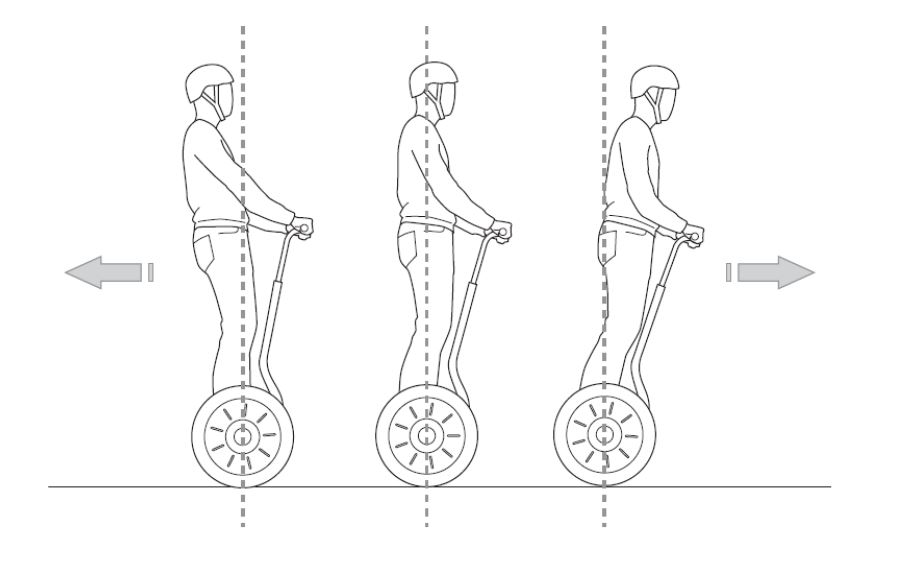
\includegraphics[width=4in]{Figures/wstep_segway.jpg}
	\captionsource{Działanie pojazdu \textit{Segway}.}{\cite{Babazadeh}}
	\label{fig:wstep_segway}
\end{figure}

Zadanie to wymaga obliczenia modelu matematycznego badanego obiektu oraz przetestowania jego działania. Następnie, na podstawie modelu, należy wyznaczyć optymalne sterowanie.